\documentclass[a5paper]{scrbook}
% !TEX ROOT = main.tex

\usepackage[ngerman]{babel}
\usepackage[utf8]{inputenc}
\usepackage{libertine}
\usepackage{libertinust1math}
\usepackage[T1]{fontenc}
\usepackage{microtype}
\usepackage{amsmath}
\usepackage{eurosym}
\usepackage[pdftex]{graphicx}
\usepackage{fancyhdr}
\usepackage{blindtext}
\usepackage{todonotes}
\usepackage{geometry}
\usepackage{url}
\usepackage{fontawesome}
\usepackage{hyperref}
\usepackage{wrapfig}
\usepackage{pdfpages}
\usepackage{tocloft}
\usepackage{subcaption}
\usepackage{paralist}

% Suche nach Grafiken in ./media und .:
\graphicspath{{./media/}{./}}

% Satzspiegel
\geometry{inner=20mm, outer=15mm, top=15mm, bottom=25mm, heightrounded, marginparwidth=37mm, marginparsep=5mm}
%\setlength{\parindent}{0pt}

%Headlines
\pagestyle{fancy}
\fancyhf{}
\renewcommand{\headrulewidth}{0pt}
%\fancyhead[LE]{\leftmark}
%\fancyhead[RO]{\rightmark}
\fancyfoot[RO,LE]{\thepage}

%Lied-Umgebung einspaltig
\newenvironment{lied}[2]%
  {\section*{#1}\textit{#2}\\\\\bgroup\footnotesize}
  {\egroup\vspace{1cm}}

%Lied-Umgebung zweispaltig mit einspaltigem Titel 
\newenvironment{lied*}[2]%
  {\twocolumn[\section*{#1}\textit{#2}\\]\bgroup\footnotesize}
  {\egroup\vspace{1cm}}  

%Lied-Umgebung komplett zweispaltig oder einspaltig jenachdem wie es davor definiert war
\newenvironment{lied**}[2]%
  {\section*{#1}\textit{#2}\\\\\bgroup\footnotesize}
  {\egroup\vspace{1cm}}    
  
%Lied-Umgebung zweispaltig ohne Untertitel
\newenvironment{lied***}[1]%
  {\twocolumn\section*{#1}\bgroup\footnotesize}
  {\egroup\vspace{1cm}}  
  
%Unterdrückt Section und Subsection Nummern, also werden nur Chapter Nummer angezeigt
  \setcounter{secnumdepth}{0}

%zusätzliche Packages nur für den Mantelbogen
\usepackage[absolute]{textpos}  % Zum Positionieren der Grafiken
\usepackage{rotating}           % Zum Drehen von Text
\setlength{\parindent}{0pt}
\usepackage{background}
\backgroundsetup{
scale=1.1,
angle=0,
opacity=1,  %% adjust
contents={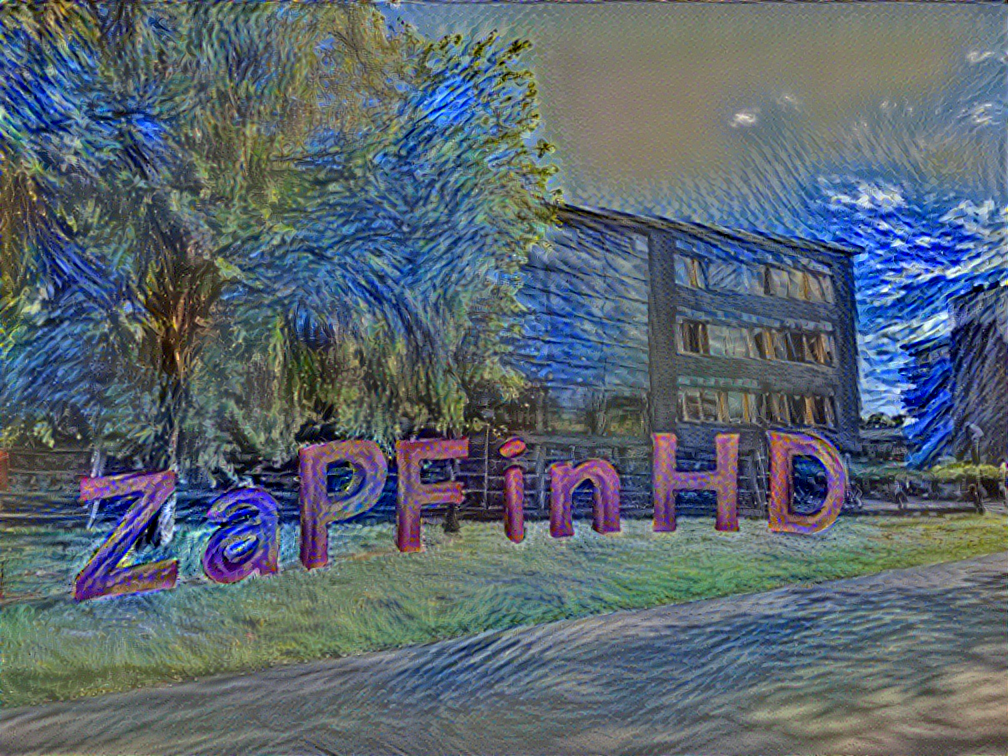
\includegraphics[width=\paperwidth]{vangogh}}
}
\usepackage{geometry}
\geometry{bottom=10mm}

\begin{document}

% VORDERSEITE, AUSSEN %
\pagestyle{empty}
\centering

\includegraphics[width=55mm]{logo_breit} 

\vspace*{14cm} \centering \fontsize{40}{48} \textbf{Tagungsheft}
\normalsize

%\begin{textblock*}{148mm}[0,0](0mm,100mm)
    %
\includegraphics[width=148mm]{logo_breit} 
%\end{textblock*}
      
% TeX denkt, dass die Seite noch leer ist und macht deswegen keinen
% pagebreak. Das \null täuscht TeX und alle sind glücklich (bis auf die
% Perfektionisten natürlich)
\null
\newpage
\backgroundsetup{
scale=1.1,
angle=0,
opacity=1,  %% adjust
contents={}
}
% VORDERSEITE, INNEN %
\vspace*{\fill}
    \begin{tabular*}{\textwidth}{ll}
        \multicolumn{2}{l}{
            \parbox{\textwidth}{
                Der Redaktionsschluss für diesen Text war am 9. Mai 2018. Wir freuen uns
                sehr über Kommentare, Anregungen, Verbesserungsvorschläge,
                Mitarbeit und Kuchen -- melde dich bei
                \href{mailto:akzapf@mathphys.stura.uni-heidelberg.de}{akzapf@mathphys.stura.uni-heidelberg.de}.
            }
            \vspace{1cm}
        }\\
	\multicolumn{2}{l}{
	\parbox{0.77\textwidth}{
       	\textbf{Bild Copyrights}
       	\begin{tabbing}
		Christoph Blattgerste \quad \quad \=  Titelbild (Cover)\\		
		Henrik Reinstädtler\> Titelbild van Gogh Stil, ÖPNV Karte\\
		Lennart Stipulkowski \> ExzellENTE, Schlossbeleuchtung, ZaPF Logo\\
		Max Häberle \> Zoo Bilder\\
		Max Menges\> 500€ gespart \\		
		VRNextbike \> Karte mit Verleihstellen\\
		OpenStreetMap \> Karte Neuenheimer Feld\\
		Samuel Scherer \> Sonnenuntergang Altstadt (Rückseite)\\
		Universität Heidelberg \> Restliche Bilder zur Geschichte\\
		\>der Fakultät und Universität\\
		

		\end{tabbing}
       	}
      }\\  
        
        \textbf{Impressum} &\\
        Herausgeber & Studienfachschaft Physik, Universität Heidelberg \\
        & Im Neuenheimer Feld 205, Raum 01.301\\
        & 69120 Heidelberg\\
        V.\,i.\,S.\,d.\,P. & Jan Gräfje\\
        & Im Neuenheimer Feld 205, Raum 01.301\\
        & 69120 Heidelberg\\
    \end{tabular*}

    \vfill

    \begin{textblock*}{203mm}[0,1](-7mm,290mm)
        \begin{flushright}
            \footnotesize
            \href{http://mathphys.info}{Coverbild: URHEBER} \href{http://creativecommons.org/licenses/by-sa/4.0/}{(CC-BY-SA)}\\  
        \end{flushright}
    \end{textblock*}



\null
\newpage

% RÜCKSEITE, INNEN %
\pagestyle{empty}
% Campusplan
\null
\backgroundsetup{
scale=1,
angle=90,
opacity=1,  %% adjust
contents={\includegraphics[width=\paperheight]{map}}
}

\newpage

% RÜCKSEITE, AUSSEN %
\pagestyle{empty}
\null
\backgroundsetup{
scale=1.06,
angle=270,
opacity=1,  %% adjust
contents={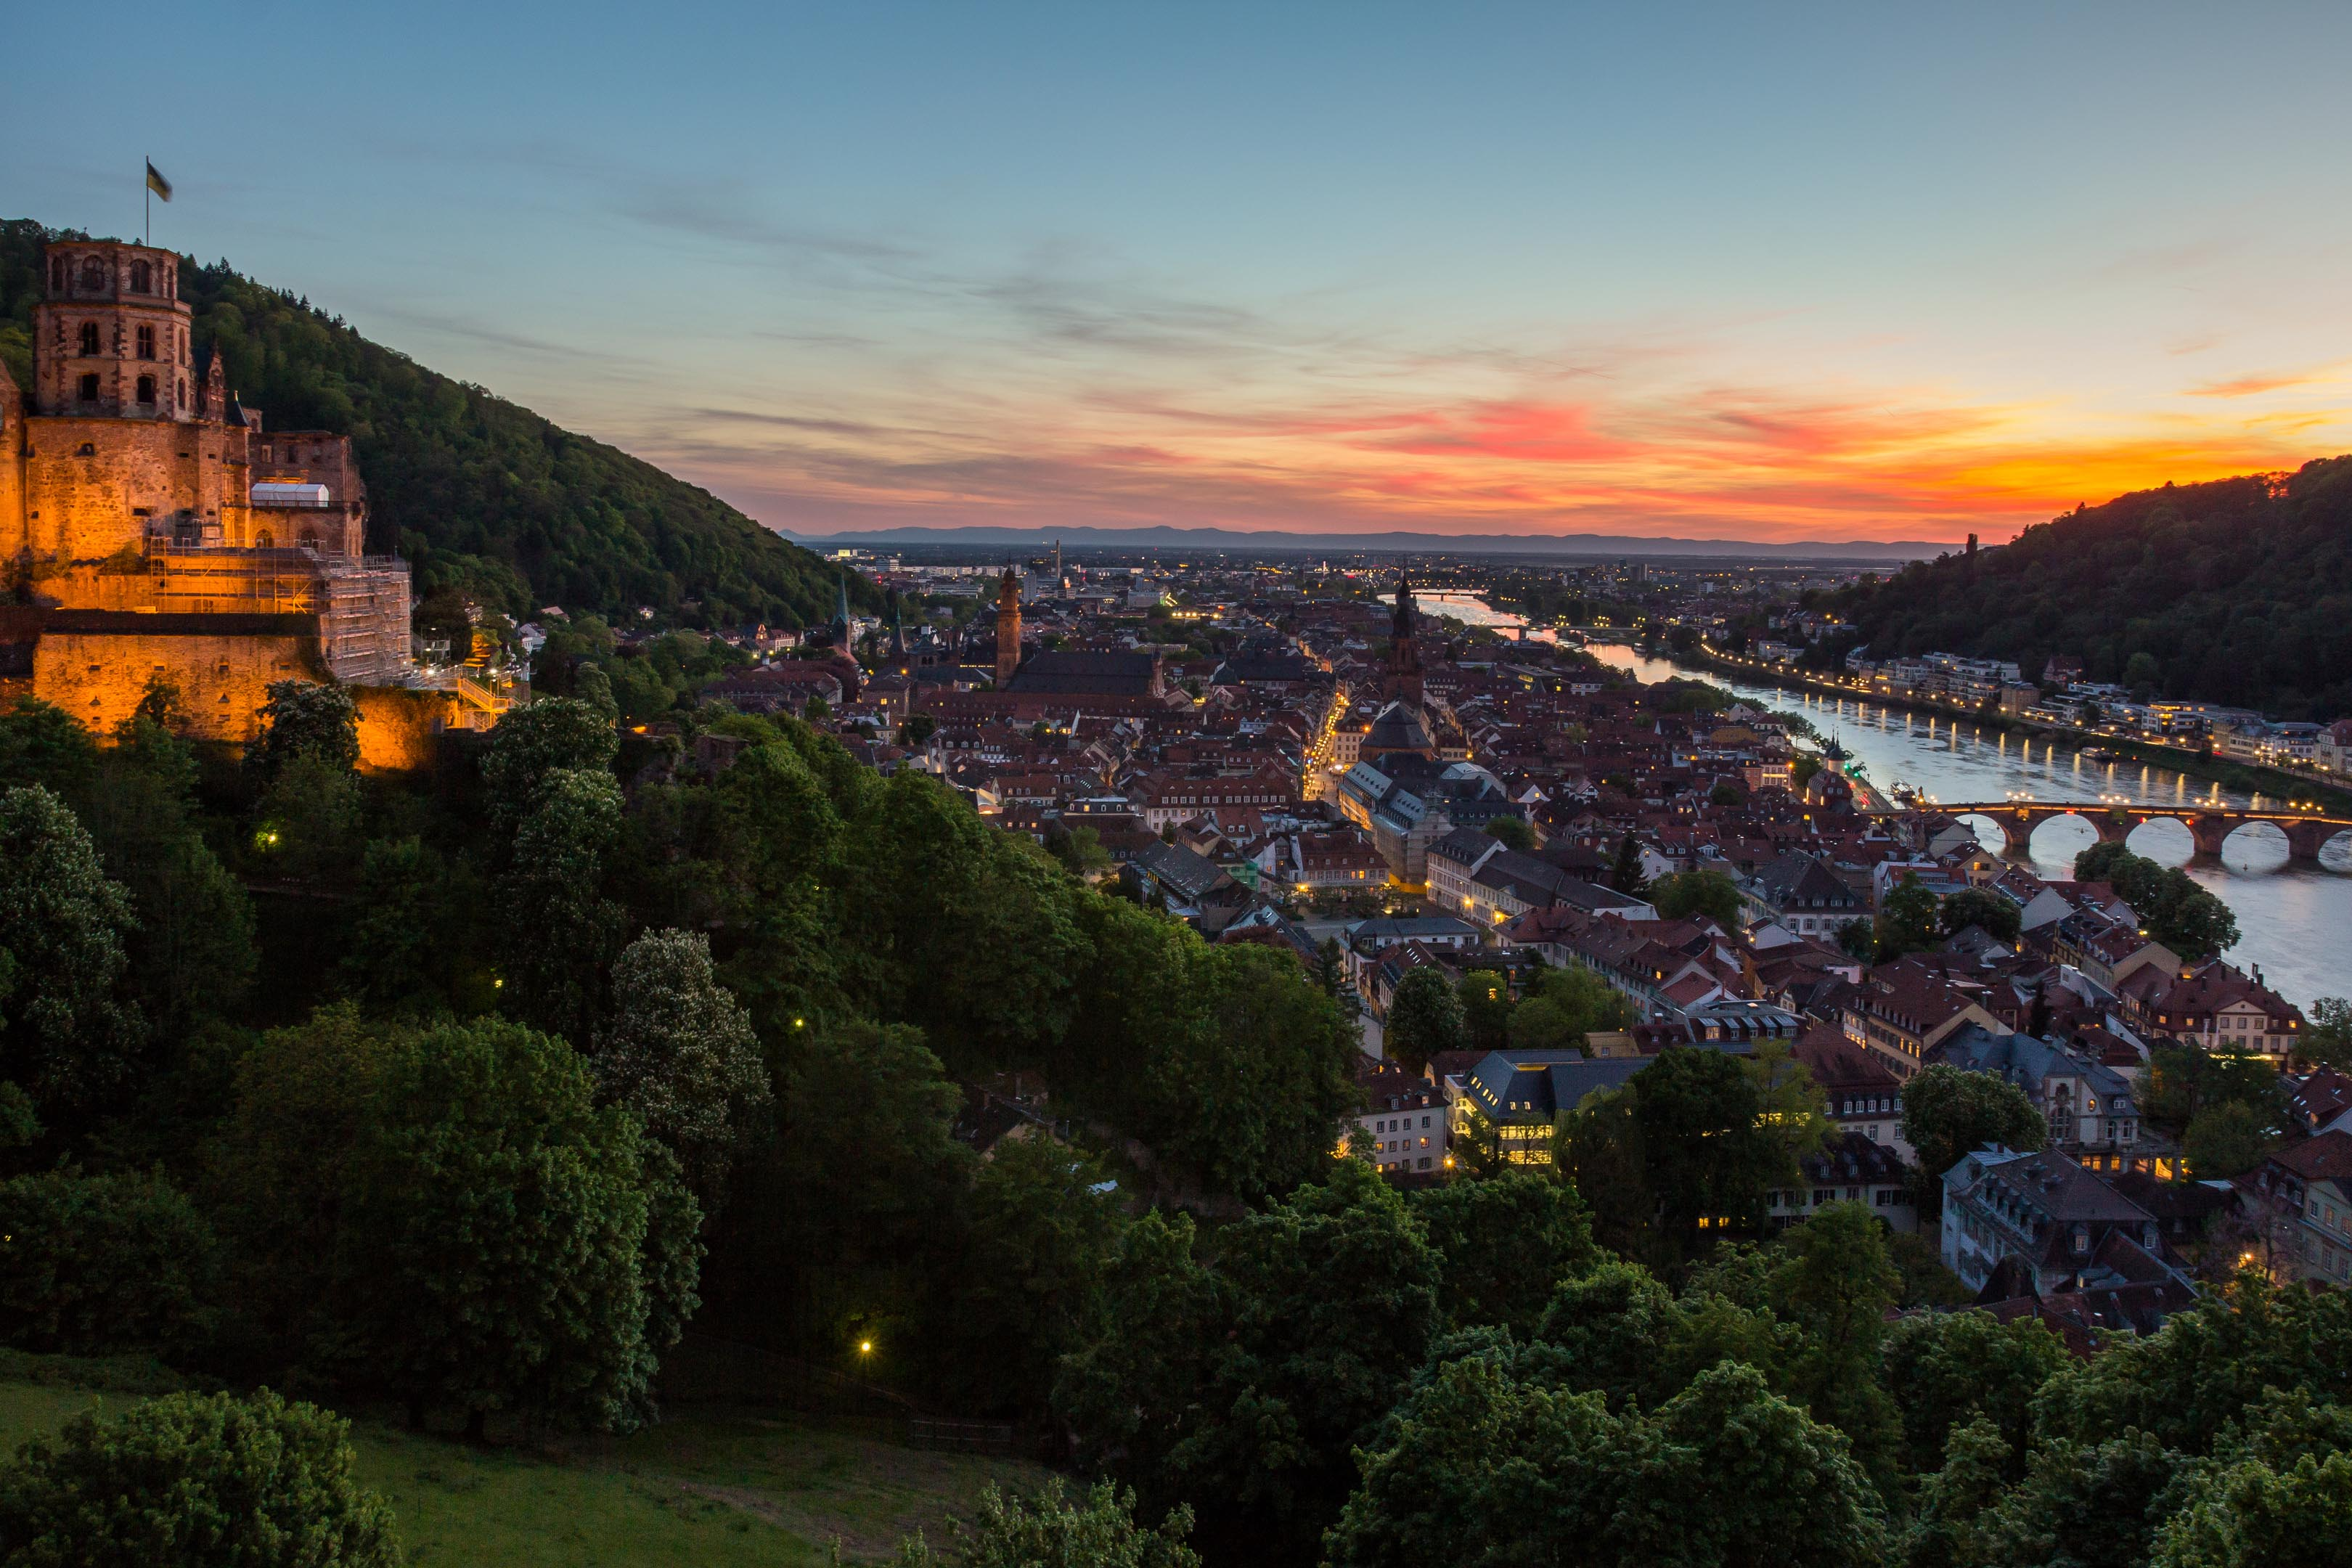
\includegraphics[width=\paperheight]{altstadt}}
}

\vspace{2cm}
\raggedright
\hspace{-1.25cm}

\includegraphics[angle=270, width=2cm]{media/exzellente}


%\begin{textblock}{30}(8.8,1)
%\includegraphics[width=50mm]{MathPhysInfoLogo} 
%\end{textblock}
\newpage
\end{document}
